\documentclass[openany]{article}
\usepackage[a4paper,margin=1in,bottom=1.5in]{geometry} % define margins. Bottom margin is used to lift a little bit the page number.
\usepackage[english]{babel} % document language is english
\usepackage{graphicx} % for including images
\usepackage[export]{adjustbox}
\usepackage{fancyhdr} % used for creating headers and footers. only used in title page in this document.
\usepackage{tabularx} % creation of more complex tables
\usepackage{longtable} % tables can span multiple pages
\usepackage{array} % allow elements of tabular environment to have vertical alignment, e.g., center alignment.
\usepackage{nameref} % make it possible to reference by name
\usepackage{hyperref} % allow hiperlinks (links to other document parts and extern links)
\usepackage{etoc} % used for generation of section local table of contents
\usepackage{placeins} % defines the \FloatBarrier command
\usepackage[dvipsnames]{xcolor} % for modifying box color
\usepackage{tikz} % for drawing (currently not used).
\usepackage{adjustbox} % for modifying box parameters
\usepackage{textcomp} % for having the degree symbol
\usepackage{listings} % for code snippets

% configure a listing environment for code snippets
\lstnewenvironment{code}
    {\lstset{linewidth=\linewidth,
             backgroundcolor=\color{white},
             frame=single,basicstyle=\normalsize\ttfamily\color{black},
             breaklines=true
             }}
    {}

% Define graphics path
\graphicspath{{figs/}}

% Configure the cross reference hyper links color
\hypersetup{
    colorlinks=true,
    linkcolor=blue,
}

\newcolumntype{C}{>{\centering\arraybackslash}X} % new column type for tabularx
                         % centered (\centering), adjust width in order to fill table width (X type)

% Configure header in 'titlepage'
\pagestyle{fancy}
\lhead{
\includegraphics[width=4.5cm]{logo_cnpem}}
\rhead{
\includegraphics[width=4cm]{logo_lnls}}
\renewcommand{\headrulewidth}{0pt}
\setlength{\headheight}{52pt}
% Clean footer
\fancyfoot{}

% increase table height factor a little bit (taller cells)
\renewcommand{\arraystretch}{1.5}

%==== Begin DOCUMENT ====
\begin{document}

%--- Begin title page ---
\begin{titlepage}

% Add header to this page
\thispagestyle{fancy}

% Center elements
\begin{center}

% title of title page
\topskip0pt % perfectly centered
\vspace*{\fill}
\textbf{\Huge Diff Ctrl EPICS IOC User Guide}\\[20pt]
\textbf{\Huge Version 1.0}\\[20pt]
\textbf{\Huge May/2020}
\vspace*{\fill}

% footer of title page
\vfill
\textbf{Beam Diagnostics Group (DIGS)}\\[5pt]
\textbf{Brazilian Synchrotron Light Laboratory (LNLS)}\\[5pt]
\textbf{Brazilian Center for Research in Energy and Materials (CNPEM)}
\end{center}

\end{titlepage}
%--- End of title page ---

\newpage
\pagestyle{plain} % restore default page style

%--- About this manual ---
\paragraph{}{\Large\bfseries About this manual}

\paragraph{} This manual provides an overview of the Diff Ctrl EPICS Soft IOC. It is assumed that the reader is familiar with the basics of EPICS.

%--- Table of contents ---
\tableofcontents

\newpage
%--- Section: Introduction ---
\section{Introduction}

\paragraph{} The Diff Ctrl EPICS IOC is a Soft IOC that controls the position of 2 'blades' or 'edges' that move in opposite directions. This IOC aims to meet the needs of different applications that could have this description. In case of Sirius, it is used for Slits and Scrapers at the accelerator. Since both systems use DMC 30017 Galil controllers, the PVs accessed by the Diff Ctrl IOC in order to command the motors of a given device are provided by (two) instances of the \href{https://github.com/lnls-dig/galil-dmc30017-epics-ioc}{Galil DMC 30017 EPICS IOC support by LNLS}.

\paragraph{} The Diff Ctrl IOC repository is \url{https://github.com/lnls-dig/diff-ctrl-epics-ioc}.

%--- Section: Installation ---
\section{Installation}

    \paragraph{Shortcut} It is possible to run a \emph{docker image} containing the IOC and all of its dependencies. Go to the \hyperref[sec:run-with-docker]{Running the IOC from a docker container} section to see how to do it.

    \subsection{Installing without docker}

        \paragraph{Before everything} Make sure you have EPICS Base 3.15 and the following EPICS modules installed (older versions might work but are not recommended):

        \begin{itemize}
          \item autosave R5-9
          \item seq 2-2-6
          \item calc R3-7
          \item busy R1-7
        \end{itemize} 

        \paragraph{} Clone the IOC repository and checkout the desired commit (in case you are not using master).

            \vspace{1mm}
            \begin{code}
git clone https://github.com/lnls-dig/diff-ctrl-epics-ioc.git <install location>
cd <install location>
git checkout <commit>
            \end{code}
            \vspace{1mm}

        \paragraph{} Create a \emph{RELEASE.local} file inside the \emph{configure/} directory and add the paths to EPICS Base and external modules. An example file is available at \emph{configure/RELEASE.local.example}.

            \vspace{1mm}
            \begin{code}
echo 'EPICS_BASE=<EPICS Base path>' > configure/RELEASE.local
echo 'AUTOSAVE=<Autosave path>' >> configure/RELEASE.local
echo 'SNCSEQ=<seq path>' >> configure/RELEASE.local
echo 'CALC=<calc path>' >> configure/RELEASE.local
echo 'BUSY=<busy path>' >> configure/RELEASE.local
            \end{code}
            \vspace{1mm}

        \paragraph{} From the IOC $<$TOP$>$ directory, run make:

            \vspace{1mm}
            \begin{code}
make
            \end{code}
            \vspace{1mm}

%--- Section: Running the IOC without docker ---
\section{Running the IOC without docker}

    After successfully building the IOC, from the IOC top directory, run:

        \vspace{1mm}
        \begin{code}
cd iocBoot/iocDiffCtrl &&
./runDiffCtrl.sh <options>
        \end{code}
        \vspace{1mm}

    The available options can be listed by passing any invalid option to the startup script, such as:

        \vspace{1mm}
        \begin{code}
./runDiffCtrl.sh -h
        \end{code}
        \vspace{1mm}

    or can be consulted in the README.md file at the IOC $<$TOP$>$ directory or project page \url{https://github.com/lnls-dig/diff-ctrl-epics-ioc}.

%--- Section: Running the IOC from a docker container ---
\section{Running the IOC from a docker container}\label{sec:run-with-docker}

    \paragraph{} Make sure you have docker installed and that you understand the basics of creating, running and acessing a container, and downloading an image.

    \subsection{Downloading the image (IOC + dependencies)}

        \paragraph{} The image named \textbf{lnlsdig/diff-ctrl-epics-ioc} contains the compiled IOC and dependencies, and can be downloaded to your machine by running:

        \vspace{1mm}
        \begin{code}
docker pull lnlsdig/diff-ctrl-epics-ioc:<IOC_TAG>
        \end{code}
        \vspace{1mm}

        where \emph{$<$IOC\_TAG$>$} should be replaced by the desired IOC version.

        \paragraph{} The IOC version list can be found at \url{https://hub.docker.com/r/lnlsdig/diff-ctrl-epics-ioc/tags}.

        After the IOC image is downloaded, you can instante it by running a container that uses it.

    \subsection{Running a docker container with that image}

        \paragraph{} One way to run the container is to do:

        \vspace{1mm}
        \begin{code}
docker run -it --network host --restart always --name <CONTAINER_NAME> lnlsdig/diff-ctrl-epics-ioc:<IOC_TAG> -P <PREFIX1> -R <PREFIX2> <other options>
        \end{code}
        \vspace{1mm}

        Which is going to run the container starting at its default entrypoint, that is, the IOC startup script. The parameter $<$IOC\_TAG$>$ should be replaced by the IOC version. All the arguments after it are passed to the IOC startup script when run in this way. The $<$PREFIX1$>$ and $<$PREFIX2$>$ are the IOC EPICS PVs prefix, combined as follows: \emph{PV\_PREFIX = PREFIX1 + PREFIX2}. The other startup script arguments should be provided as well. They are listed in the IOC README.md file.

        \paragraph{} \textbf{If you run this command before downloading the image, the image is automatically downloaded, provided there is internet connection}.

        \paragraph{} Below you find an explanation for each flag we used in the above command.

        \begin{itemize}
          \item -it: interactive (STDIN open) and allocate pseudo-TTY. Since we did not change the container entrypoint, your terminal is going to connect to the IOC shell.
          \item --network host: configures the container to use the host's network stack inside the container. It is the simplest configuration to use, although it provides no isolation.
          \item --restart always: restarts the container automatically when it exits.
          \item --name $<$CONTAINER\_NAME$>$: configures the container name as $<$CONTAINER\_NAME$>$.
        \end{itemize}

        \paragraph{} In order to stop the docker container, i.e., the IOC, run:

        \vspace{1mm}
        \begin{code}
docker stop <CONTAINER_NAME>
        \end{code}
        \vspace{1mm}

        \paragraph{} If you want to delete the container, after stopping it, run:

        \vspace{1mm}
        \begin{code}
docker rm <CONTAINER_NAME>
        \end{code}
        \vspace{1mm}

        \paragraph{} You can also run the contaier with the \emph{--rm} flag to clean up the container and remove the file system when it exits.

%--- Section: Device Reference Frame ---
\section{Device Reference Frame}\label{sec:dev-reference-frame}

    \paragraph{} The IOC control follows the beam coordinate system. This means the X axis increments in value from right to left (greater beam energy) and the Y axis increments in value from bottom to top.

    \paragraph{} The origin of the X and Y axis is considered to be at the device center. If the beam passes through the 0 position, this means it is perfectly centered with respect to the device.

    \paragraph{} The device blade, or edge, that when retreated is positioned in the negative region of the X axis (or Y axis) is refered to as the \emph{Negative Edge}.

    \paragraph{} The device blade, or edge, that when retreated is positioned in the positive region of the X axis (or Y axis) is refered to as the \emph{Positive Edge}.

    \paragraph{} The figure \ref{fig:ref-frame} illustrates the positioning of the blades (edges) considering some coordinates.

    \begin{figure}[!h]
        \caption{Device reference frame overview}
        \label{fig:ref-frame}
        \centering
        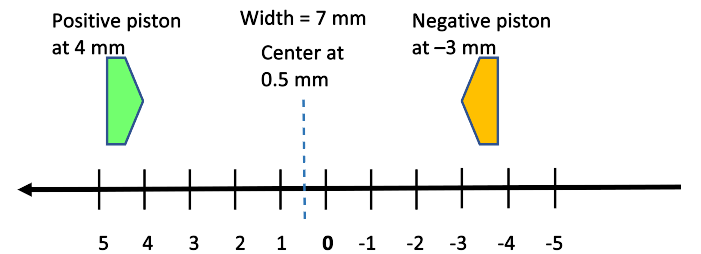
\includegraphics[width=1.0\textwidth]{diff_ctrl_ref_frame}
    \end{figure}
    \FloatBarrier


%--- Section: Edge Control Overview ---
\section{Edge Control Overview}

    \paragraph{} Following a common way of implementing Slit control, the user can control the device by either specifying each blade position (in the device reference frame) or provide the slit center position and width. Figure \ref{fig:ref-frame} illustrates these parameters.

    \paragraph{} Figure \ref{fig:opi-overview} shows the Diff-Ctrl CS-Studio OPI with the main features circled. The green circles show where the \emph{Negative} and \emph{Positive} edge positions can be specified. The red circles show where the gap center and width should be specified.

    \begin{figure}[!h]
        \caption{OPI overview}
        \label{fig:opi-overview}
        \centering
        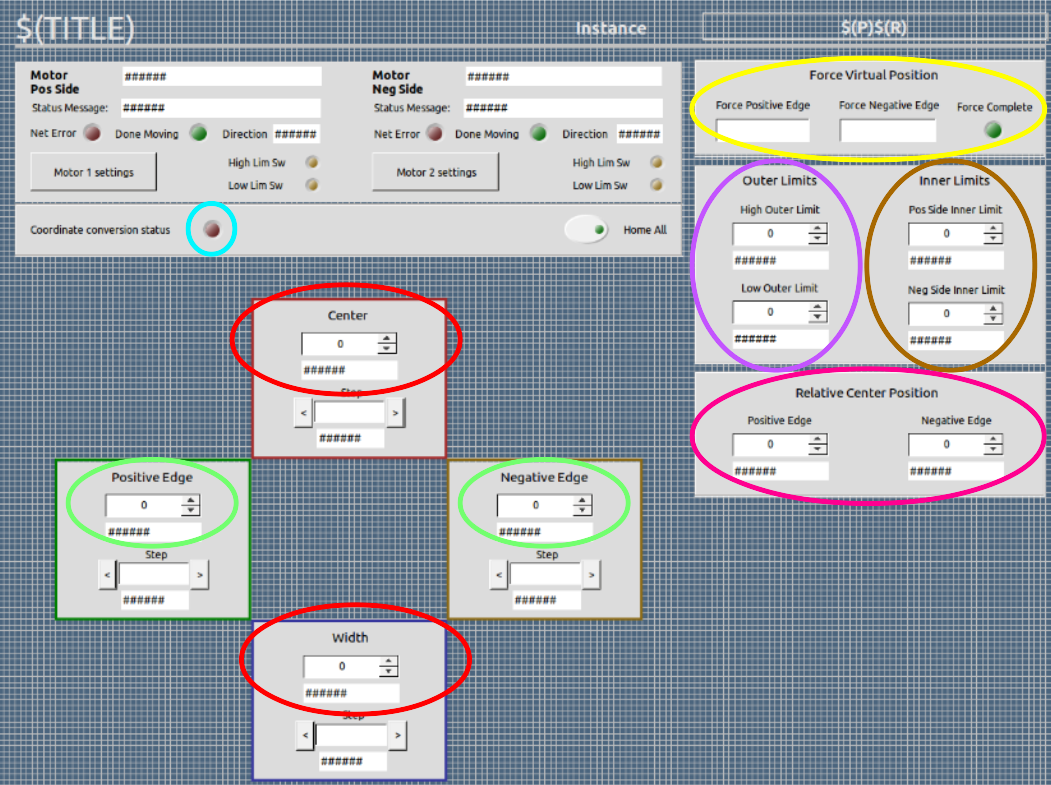
\includegraphics[width=1.0\textwidth]{diff_ctrl_OPI}
    \end{figure}
    \FloatBarrier

%--- Section: Edge Position Calibration ---
\section{Edge Position Calibration}\label{sec:edge-pos-cal}

    \paragraph{} The readback position of the blades can be calibrated to account for encoder offsets. The yellow circle in Figure \ref{fig:opi-overview} shows the \emph{Force Position} fields. These fields allow the user to force a desired readback position to a blade (or edge). When a value is set, the \emph{Force Complete} LED turns off while the force operation is in progress. When the force operation is complete, the LED turns on again. Only one edge position can be forced at a time. The value should be specified in engineering units.

    \bigskip
    \noindent\adjustbox{minipage=\textwidth,cfbox=red 1.0pt 2ex}{
        The \emph{Force Position} command can only compensate offsets to the encoder values. It cannot compensate for deviations in the device motion, since this is encoded in the motor-edge conversion function applied for each edge. To understand how to compensate for fixed offsets in edge position, see section \nameref{sec:ref-center-cal}.
    }

%--- Section: Configuring Software Limits ---
\section{Configuring Software Limits}

    \paragraph{} This IOC should control a device with 2 actuators. This means there can be 4 limits to the device motion, that is, 2 for each blade.

    \paragraph{} The limits to the blade retreat motion are referred to as \emph{Outer Limits}, since they are associated with limiting the opening of the device gap. The limits to the blades "advance" motion are referred to as \emph{Inner Limits}, since they refer to limits for the gap closing. The "retreat" and "advance" terms refer only to the motion of parts that can interact with the beam, that is, the blades themselves. Any coordinate conversion between motors and blade position should not be considered here.

    \paragraph{} The Figure \ref{fig:outer-limits} illustrates how the outer limits configuration affects motion.

    \begin{figure}[!h]
        \caption{Outer limits}
        \label{fig:outer-limits}
        \centering
        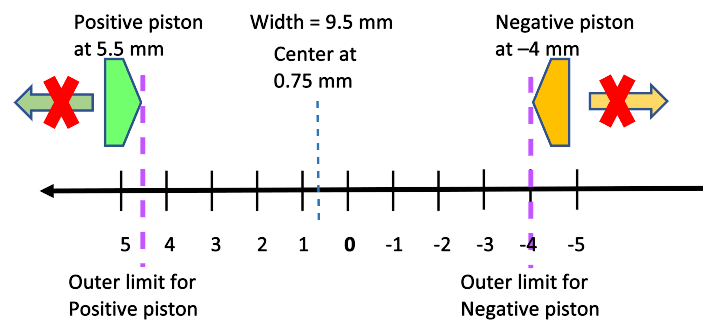
\includegraphics[width=1.0\textwidth]{diff_ctrl_outer_limits}
    \end{figure}
    \FloatBarrier

    \paragraph{} The Figure \ref{fig:inner-limits} illustrates how the inner limits configuration affects motion.

    \begin{figure}[!h]
        \caption{Inner limits}
        \label{fig:inner-limits}
        \centering
        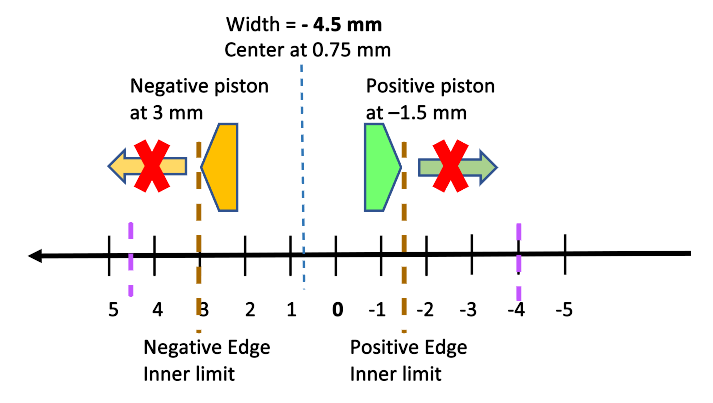
\includegraphics[width=1.0\textwidth]{diff_ctrl_inner_limits}
    \end{figure}
    \FloatBarrier

    \paragraph{} In Figure \ref{fig:opi-overview}, the \emph{Outer Limits} configuration fields are circled in purple, while the \emph{Inner Limits} configuration fields are circled in brown.

%--- Section: Reference Center Calibration ---
\section{Reference Center Calibration}\label{sec:ref-center-cal}

    \paragraph{} In addition to the \hyperref[sec:edge-pos-cal]{calibration of the offset of encoder readings}, it is also possible to configure an additional offset for edge position. When a position is forced for encoder calibration, the resulting encoder offset is considered when converting the motor position into the blade position through the selected \hyperref[sec:ref-frame-conv]{coordinate conversion function}. The \emph{Center Offset} can be used to shift the blade position reading, ignoring the underlying conversion function between motor and blade coordinates.

    \paragraph{} The Figure \ref{fig:offset-cal} shows the difference between the \emph{Reference Center Offset} and the \emph{Encoder Offset}. While the \emph{Encoder Offset} shifts the position along the conversion function curve, the \emph{Reference Center Offset} shifts the blade position directly away or towards the device center position, while keeping the encoder readback unchanged. This means that each blade coordinate conversion function input is kept unchanged.

    \paragraph{} The \emph{Center Offset} is useful for compensating offsets due to device misalignment (the device center does not match the vacuum chamber center) without the need to modify the conversion functions code.

    \begin{figure}[!h]
        \caption{Offset types}
        \label{fig:offset-cal}
        \centering
        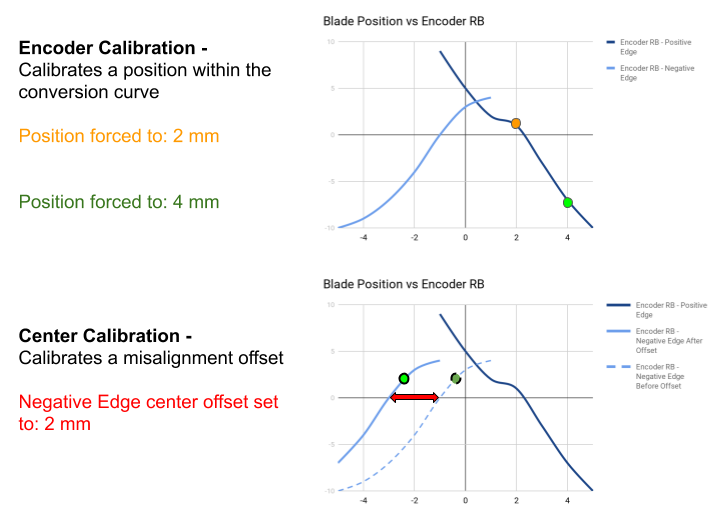
\includegraphics[width=1.0\textwidth]{diff_ctrl_offset_cal}
    \end{figure}
    \FloatBarrier

    \paragraph{} The Figures \ref{fig:reference-center-1} and \ref{fig:reference-center-2} illustrate how the \emph{Center Offset} value affects the position values. Greater offset values virtually "retreat" the edge with respect to the device center. Figure \ref{fig:reference-center-2} shows offsets configured for blades that have moved beyond the center position (the effect is the same, but retreating puts the edge closer to the center). Negative offset values do the opposite, "moving" the blades in the advancing direction.

    \begin{figure}[!h]
        \caption{Reference Center Example - blades retreated}
        \label{fig:reference-center-1}
        \centering
        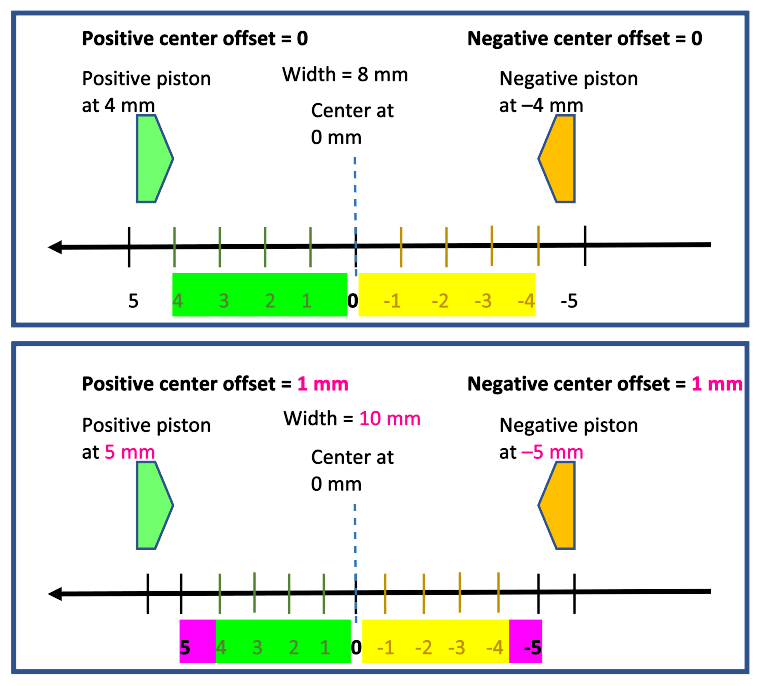
\includegraphics[width=1.0\textwidth]{diff_ctrl_reference_center_1}
    \end{figure}
    \FloatBarrier

    \begin{figure}[!h]
        \caption{Reference Center Example - blades advanced past center}
        \label{fig:reference-center-2}
        \centering
        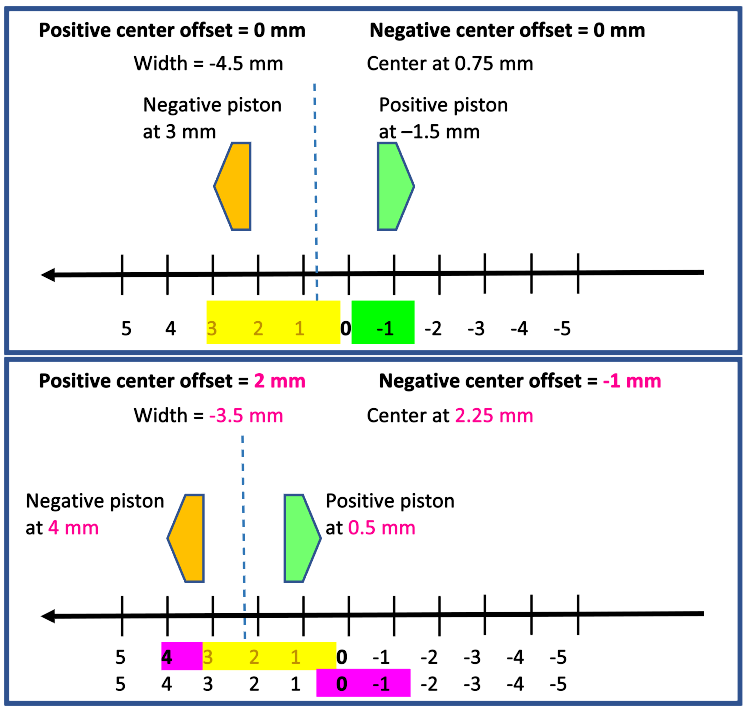
\includegraphics[width=1.0\textwidth]{diff_ctrl_reference_center_2}
    \end{figure}
    \FloatBarrier

%--- Section: Reference Frame Conversion ---
\section{Motor vs Blade Reference Frame Conversion}\label{sec:ref-frame-conv}

    This document is still under development.

%--- Section: How to Add a New Conversion Type ---
\section{How to Add a New Conversion Type}

    This document is still under development.

\newpage
\section{Process Variables Description}\label{sec:process-variables}

    Each IOC instance should add a prefix to the process variables indicating which device it controls.

    % Process Variables description table
    \begin{longtable}{| m{4.5cm} m{2.5cm}  m{7.0cm} |}
        \caption{Application Process Variables} \\ \hline
        \bfseries Name & \bfseries Data Type & \bfseries Description \label{tab:PV-description} \endfirsthead
        \caption{Application Process Variables} \\ \hline
        \bfseries Name & \bfseries Data Type & \bfseries Description \endhead \hline
        % --- row ---
        PV\_NAME & DATA\_TYPE & \begin{tabular}{@{}m{6cm}@{}}
                            DESCRIPTION
            \end{tabular} \hypertarget{pv:negative-motion-ctrl-cte}{}\\ \hline
        % --- row ---
        NegativeMotionCtrl-Cte & String (char[40]) & \begin{tabular}{@{}m{6cm}@{}}
                Prefix used for device \emph{negative edge} motion controller.
            \end{tabular} \hypertarget{pv:positive-motion-ctrl-cte}{}\\ \hline
        % --- row ---
        PositiveMotionCtrl-Cte & String (char[40]) & \begin{tabular}{@{}m{6cm}@{}}
                Prefix used for device \emph{positive edge} motion controller..
            \end{tabular} \hypertarget{pv:negative-done-mov-mon}{}\\ \hline
        % --- row ---
        NegativeDoneMov-Mon & Enum: No (0) Yes (1) & \begin{tabular}{@{}m{6cm}@{}}
                Indicates when the \emph{negative edge} is done moving, i.e., when it has completely finished its motion.
            \end{tabular} \hypertarget{pv:positive-done-mov-mon}{}\\ \hline
        % --- row ---
        PositiveDoneMov-Mon & Enum: No (0) Yes (1) & \begin{tabular}{@{}m{6cm}@{}}
                Indicates when the \emph{positive edge} is done moving, i.e., when it has completely finished its motion.
            \end{tabular} \hypertarget{pv:negative-edge-pos}{}\\ \hline
        % --- row ---
        NegativeEdgePos-SP & Float: min -1e6, max 1e6 & \begin{tabular}{@{}m{6cm}@{}}
                Command the \emph{negative edge} to move to the specified distance, in engineering units, from the \emph{reference axis center}. More information on the device reference frame convention can be found in section \nameref{sec:dev-reference-frame}. This PV does not necessarily indicate the current edge position, for that, the readback value should be used.
            \end{tabular} \hypertarget{}{}\\ \hline
        % --- row ---
        NegativeEdgePos-RB & Float & \begin{tabular}{@{}m{6cm}@{}}
                Shows the \emph{negative edge} distance, in engineering units, from the \emph{reference axis center}. This value is updated whenever the edge encoder registers a movement.
            \end{tabular} \hypertarget{pv:positive-edge-pos}{}\\ \hline
        % --- row ---
        PositiveEdgePos-SP & Float: min -1e6, max 1e6 & \begin{tabular}{@{}m{6cm}@{}}
                Command the \emph{positive edge} to move to the specified distance, in engineering units, from the \emph{reference axis center}. More information on the device reference frame convention can be found in section \nameref{sec:dev-reference-frame}. This PV does not necessarily indicate the current edge position, for that, the readback value should be used.
            \end{tabular} \hypertarget{}{}\\ \hline
        % --- row ---
        PositiveEdgePos-RB & Float & \begin{tabular}{@{}m{6cm}@{}}
                Shows the \emph{positive edge} distance, in engineering units, from the \emph{reference axis center}. This value is updated whenever the edge encoder registers a movement.
            \end{tabular} \hypertarget{pv:center}{}\\ \hline
        % --- row ---
        Center-SP & Float & \begin{tabular}{@{}m{6cm}@{}}
                Command both the \emph{positive and negative edges} movement so that the midpoint between them is located at the specified distance, in engineering units, from the \emph{reference axis center}. More information on the device reference frame convention can be found in section \nameref{sec:dev-reference-frame}. This PV does not necessarily indicate the current center position, for that, the readback value should be used.
            \end{tabular} \hypertarget{}{}\\ \hline
        % --- row ---
        Center-RB & Float & \begin{tabular}{@{}m{6cm}@{}}
                Shows the distance of the midpoint between the \emph{positive and negative edges}, in engineering units, from the \emph{reference axis center}. This value is updated whenever the encoder of one of the edges registers a movement.
            \end{tabular} \hypertarget{pv:width}{}\\ \hline
        % --- row ---
        Width-SP & Float & \begin{tabular}{@{}m{6cm}@{}}
                Command both the \emph{positive and negative edges} movement so that the distance between them is set to the specified value, in engineering units. They edges are moved in such a way that keeps the \emph{Center-RB} position unchanged. More information on the device reference frame convention can be found in section \nameref{sec:dev-reference-frame}. This PV does not necessarily indicate the current width between the edges, for that, the readback value should be used.
            \end{tabular} \hypertarget{}{}\\ \hline
        % --- row ---
        Width-RB & Float & \begin{tabular}{@{}m{6cm}@{}}
                Shows the distance between the \emph{positive and negative edges}, in engineering units. This value is updated whenever the encoder of one of the edges registers a movement.
            \end{tabular} \hypertarget{pv:coord-conv-err-mon}{}\\ \hline
        % --- row ---
        CoordConvErr-Mon & Enum: Ok (0), Error (1) & \begin{tabular}{@{}m{6cm}@{}}
                Error status of the coordinate conversion between encoder reading and actual edge position. If the error status is 1, then the conversion function failed for the given commanded position or for the current encoder reading. This can be due to invalid input, for instance, an out of range position, or to some error in the function itself.
            \end{tabular} \hypertarget{pv:neg-edge-inner-lim}{}\\ \hline
        % --- row ---
        NegEdgeInnerLim-SP & Float: min -1e6, max 1e6 & \begin{tabular}{@{}m{6cm}@{}}
                The inner limit associated to the \emph{negative edge}, in engineering units. This is the limit position when moving this edge toward the reference center from the retreat position. The \emph{negative edge} retreat position is usually negative, but if the edge keeps advancing, it eventually arrives at a positive position. Thus, if the \emph{negative edge} inner limit is positive, the \emph{negative edge} can move beyond the reference center, until it reaches the specified limit. If it is negative, the edge can move torwards the center until it reaches the specified limit.
            \end{tabular} \hypertarget{}{}\\ \hline
        % --- row ---
        NegEdgeInnerLim-RB & Float & \begin{tabular}{@{}m{6cm}@{}}
                The readback value of the \emph{negative edge} inner limit.
            \end{tabular} \hypertarget{pv:pos-edge-inner-lim}{}\\ \hline
        % --- row ---
        PosEdgeInnerLim-SP & Float: min -1e6, max 1e6 & \begin{tabular}{@{}m{6cm}@{}}
                The inner limit associated to the \emph{positive edge}, in engineering units. This is the limit position when moving this edge toward the reference center from the retreat position. The \emph{positive edge} retreat position is usually positive, but if the edge keeps advancing, it eventually arrives at a negative position. Thus, if the \emph{positive edge} inner limit is negative, the \emph{positive edge} can move beyond the reference center, until it reaches the specified limit. If it is positive, the edge can move torwards the center until it reaches the specified limit.
            \end{tabular} \hypertarget{}{}\\ \hline
        % --- row ---
        PosEdgeInnerLim-RB & Float & \begin{tabular}{@{}m{6cm}@{}}
                The readback value of the \emph{positive edge} inner limit.
            \end{tabular} \hypertarget{pv:low-outer-lim}{}\\ \hline
        % --- row ---
        LowOuterLim-SP & Float: min -1e6, max 1e6 & \begin{tabular}{@{}m{6cm}@{}}
                The outer limit associated to the \emph{negative edge}, in engineering units. This is the limit retreat position for the \emph{negative edge}, i.e., the most negative position this edge can have.
            \end{tabular} \hypertarget{}{}\\ \hline
        % --- row ---
        LowOuterLim-RB & Float & \begin{tabular}{@{}m{6cm}@{}}
                The readback value of the \emph{negative edge} outer limit.
            \end{tabular} \hypertarget{pv:high-outer-lim}{}\\ \hline
        % --- row ---
        HighOuterLim-SP & Float: min -1e6, max 1e6 & \begin{tabular}{@{}m{6cm}@{}}
                The outer limit associated to the \emph{positive edge}, in engineering units. This is the limit retreat position for the \emph{positive edge}, i.e., the most positive position this edge can have.
            \end{tabular} \hypertarget{}{}\\ \hline
        % --- row ---
        HighOuterLim-RB & Float & \begin{tabular}{@{}m{6cm}@{}}
                The readback value of the \emph{positive edge} outer limit.
            \end{tabular} \hypertarget{pv:positive-edge-center}{}\\ \hline
        % --- row ---
        PositiveEdgeCenter-SP & Float & \begin{tabular}{@{}m{6cm}@{}}
                The distance between the \emph{positive edge} and the reference center. A greater distance value shifts the available positions for the \emph{positive edge} in the positive direction (greater edge position values). Smaller distance values do the opposite, including negative values.
            \end{tabular} \hypertarget{}{}\\ \hline
        % --- row ---
        PositiveEdgeCenter-RB & Float & \begin{tabular}{@{}m{6cm}@{}}
                The readback value of the distance between the \emph{positive edge} and the reference center.
            \end{tabular} \hypertarget{pv:negative-edge-center}{}\\ \hline
        % --- row ---
        NegativeEdgeCenter-SP & Float & \begin{tabular}{@{}m{6cm}@{}}
                The distance between the \emph{negative edge} and the reference center. A greater distance value shifts the available positions for the \emph{negative edge} in the negative direction (smaller edge position values). Smaller distance values do the opposite, including negative values.
            \end{tabular} \hypertarget{}{}\\ \hline
        % --- row ---
        NegativeEdgeCenter-RB & Float & \begin{tabular}{@{}m{6cm}@{}}
                The readback value of the distance between the \emph{negative edge} and the reference center.
            \end{tabular} \hypertarget{pv:force-negative-edge-pos-cmd}{}\\ \hline
        % --- row ---
        ForceNegativeEdgePos-Cmd & Float & \begin{tabular}{@{}m{6cm}@{}}
                Force a given position reading, in engineering units, to the \emph{negative edge} (does not move the edge). This is useful for calibration of the edge positions. For instance, if the change of an enconder shifts the absolute readings, but a known position can be restored (by other measurement or by a reference such as a limit switch), then the known position can be forced. The IOC does this by setting an offset to the motion controller's encoder readings.
            \end{tabular} \hypertarget{pv:force-positive-edge-pos-cmd}{}\\ \hline
        % --- row ---
        ForcePositiveEdgePos-Cmd & Float & \begin{tabular}{@{}m{6cm}@{}}
                Force a given position reading, in engineering units, to the \emph{positive edge} (does not move the edge). This is useful for calibration of the edge positions. For instance, if the change of an enconder shifts the absolute readings, but a known position can be restored (by other measurement or by a reference such as a limit switch), then the known position can be forced. The IOC does this by setting an offset to the motion controller's encoder readings.
            \end{tabular} \hypertarget{pv:force-complete-mon}{}\\ \hline
        % --- row ---
        ForceComplete-Mon & Enum: No (0), Yes (1) & \begin{tabular}{@{}m{6cm}@{}}
                Completion status of the force operation. After a position reading is forced to some of the edges, the IOC takes some time to apply the configuration. When the new offset configuration is finished, this PV goes to 1.
            \end{tabular} \hypertarget{pv:home-cmd}{}\\ \hline
        % --- row ---
        Home-Cmd & Enum: Off (0), On (1) & \begin{tabular}{@{}m{6cm}@{}}
                Command both edges to the retreat position. The \emph{positive edge} moves in the positive direction, until it hits a limit switch, while the \emph{negative edge} moves to the negative direction, until it hits a limit switch.
            \end{tabular} \hypertarget{pv:home-done-mon}{}\\ \hline
        % --- row ---
        HomeDone-Mon & Enum: In Progress (0), Finished (1), Error (2) & \begin{tabular}{@{}m{6cm}@{}}
                Homing procedure status. Indicates when the homing procedure is finished. If the procedure stops before both edges hit the home position, the PV indicates \emph{Error}.
            \end{tabular} \hypertarget{pv:positive-edge-step}{}\\ \hline
        % --- row ---
        PositiveEdgeStep-SP & Float: min -1e6, max 1e6 & \begin{tabular}{@{}m{6cm}@{}}
                The step size, in engineering units, to use \emph{positive edge} when an increment or decrement \emph{positive edge} position command is issued. See \hyperlink{pv:inc-positive-edge-cmd}{IncPositiveEdge-Cmd} and \hyperlink{pv:dec-positive-edge-cmd}{DecPositiveEdge-Cmd}.
            \end{tabular} \hypertarget{}{}\\ \hline
        % --- row ---
        PositiveEdgeStep-RB & Float & \begin{tabular}{@{}m{6cm}@{}}
                The readback value of the \emph{positive edge} step.
            \end{tabular} \hypertarget{pv:negative-edge-step}{}\\ \hline
        % --- row ---
        NegativeEdgeStep-SP & Float: min -1e6, max 1e6 & \begin{tabular}{@{}m{6cm}@{}}
                The step size, in engineering units, to use when an increment or decrement \emph{negative edge} position command is issued. See \hyperlink{pv:inc-negative-edge-cmd}{IncNegativeEdge-Cmd} and \hyperlink{pv:dec-negative-edge-cmd}{DecNegativeEdge-Cmd}.
            \end{tabular} \hypertarget{}{}\\ \hline
        % --- row ---
        NegativeEdgeStep-RB & Float & \begin{tabular}{@{}m{6cm}@{}}
                The readback value of the \emph{negative edge} step.
            \end{tabular} \hypertarget{pv:center-step}{}\\ \hline
        % --- row ---
        CenterStep-SP & Float: min -1e6, max 1e6 & \begin{tabular}{@{}m{6cm}@{}}
                The step size, in engineering units, to use when an increment or decrement \emph{center} position command is issued. See \hyperlink{pv:inc-center-cmd}{IncCenter-Cmd} and \hyperlink{pv:dec-center-cmd}{DecCenter-Cmd}.
            \end{tabular} \hypertarget{}{}\\ \hline
        % --- row ---
        CenterStep-RB & Float & \begin{tabular}{@{}m{6cm}@{}}
                The readback value of the \emph{center} step.
            \end{tabular} \hypertarget{pv:width-step}{}\\ \hline
        % --- row ---
        WidthStep-SP & Float: min -1e6, max 1e6 & \begin{tabular}{@{}m{6cm}@{}}
                The step size, in engineering units, to use when an increment or decrement \emph{width} command is issued. See \hyperlink{pv:inc-width-cmd}{IncWidth-Cmd} and \hyperlink{pv:dec-width-cmd}{DecWidth-Cmd}.
            \end{tabular} \hypertarget{}{}\\ \hline
        % --- row ---
        WidthStep-RB & Float & \begin{tabular}{@{}m{6cm}@{}}
                The readback value of the \emph{width} step.
            \end{tabular} \hypertarget{pv:inc-positive-edge-cmd}{}\\ \hline
        % --- row ---
        IncPositiveEdge-Cmd & Enum: Off (0), On (1) & \begin{tabular}{@{}m{6cm}@{}}
                Increment the \emph{positive edge} position by the step specified by \hyperlink{pv:positive-edge-step}{PositiveEdgeStep-RB}.
            \end{tabular} \hypertarget{pv:dec-positive-edge-cmd}{}\\ \hline
        % --- row ---
        DecPositiveEdge-Cmd & Enum: Off (0), On (1) & \begin{tabular}{@{}m{6cm}@{}}
                Decrement the \emph{positive edge} position by the step specified by \hyperlink{pv:positive-edge-step}{PositiveEdgeStep-RB}.
            \end{tabular} \hypertarget{pv:inc-negative-edge-cmd}{}\\ \hline
        % --- row ---
        IncNegativeEdge-Cmd & Enum: Off (0), On (1) & \begin{tabular}{@{}m{6cm}@{}}
                Increment the \emph{negative edge} position by the step specified by \hyperlink{pv:negative-edge-step}{NegativeEdgeStep-RB}.
            \end{tabular} \hypertarget{pv:dec-negative-edge-cmd}{}\\ \hline
        % --- row ---
        DecNegativeEdge-Cmd & Enum: Off (0), On (1) & \begin{tabular}{@{}m{6cm}@{}}
                Decrement the \emph{negative edge} position by the step specified by \hyperlink{pv:negative-edge-step}{NegativeEdgeStep-RB}.
            \end{tabular} \hypertarget{pv:inc-center-cmd}{}\\ \hline
        % --- row ---
        IncCenter-Cmd & Enum: Off (0), On (1) & \begin{tabular}{@{}m{6cm}@{}}
                Increment the \emph{center} position by the step specified by \hyperlink{pv:center-step}{CenterStep-RB}.
            \end{tabular} \hypertarget{pv:dec-center-cmd}{}\\ \hline
        % --- row ---
        DecCenter-Cmd & Enum: Off (0), On (1) & \begin{tabular}{@{}m{6cm}@{}}
                Decrement the \emph{center} position by the step specified by \hyperlink{pv:center-step}{CenterStep-RB}.
            \end{tabular} \hypertarget{pv:inc-width-cmd}{}\\ \hline
        % --- row ---
        IncWidth-Cmd & Enum: Off (0), On (1) & \begin{tabular}{@{}m{6cm}@{}}
                Increment the \emph{width} by the step specified by \hyperlink{pv:width-step}{WidthStep-RB}.
            \end{tabular} \hypertarget{pv:dec-width-cmd}{}\\ \hline
        % --- row ---
        DecWidth-Cmd & Enum: Off (0), On (1) & \begin{tabular}{@{}m{6cm}@{}}
                Decrement the \emph{width} by the step specified by \hyperlink{pv:width-step}{WidthStep-RB}.
            \end{tabular} \hypertarget{}{}\\ \hline
    \end{longtable}

\end{document}
\grid

